\chapter{Ledjes}\label{chap:ledjes}
In de introductie heb je kennis gemaakt met CircuitPython en Mu editor en heb je een ledje op het bordje zelf aangestuurd. Een micro-controller wordt voornamelijk gebruikt om externe hardware aan te sturen. In dit hoofdstuk worden ledjes op verschillende manieren aangestuurd. Een ledje laten branden is niet heel spannend, maar het is \'e\'en van de simpelste manieren om code te testen. Het maken van een led circuit is erg eenvoudig en je krijgt gelijk visuele feedback. Ook zit tussen het aansturen van een ledje of een motor weinig verschil.

\newpage
\section{Extern LEDje laten branden}\label{sec:ledExtern}
	\paragraph{Probleem:} Je wilt een externe LED laten knipperen.
	\paragraph{Benodigdheden:}
	\begin{itemize}
		\item 1x LED
		\item 1x \SI{680}{\ohm} weerstand (Of weerstand die in de buurt komt)
	\end{itemize}
	\paragraph{Oplossing:}
		\begin{figure}[H]
			\center{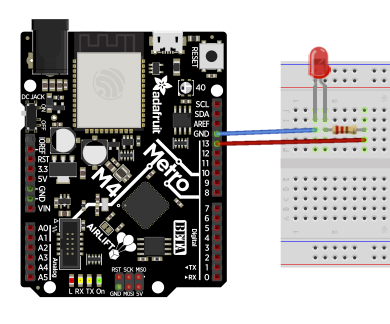
\includegraphics[width=0.6\linewidth]{figures/LED.png}}
			\caption{Led Circuit}
			\label{fig:LED}
		\end{figure}
		\lstinputlisting{code/LED.py}

	\paragraph{Discussie:}  Om een ledje te laten knipperen zijn drie modules nodig. De "board" module, zodat de pinnen aangeroepen kunnen worden met het nummer dat op het bordje staat. De "time" module om gebruik te kunnen maken van tijd en timing functies en de digitalio module zodat de I/O pinnen ingesteld kunnen worden. \\
	
	De LED zit aangesloten op pin 13 en kan daarom aan en uit gezet worden door de spanning op pin 13 hoog en laag te zetten. In de code kan je controle krijgen over pin 13 met het gebruik van de DigitalInOut() functie van de digitalio module. De functie neemt als parameter het nummer van de pin dat je wilt gebruiken en cre\"eert dan een 'object', zodat je pin 13 met code kan aansturen. In de code krijgt het object de naam led toegewezen. Een I/O pin kan zowel voor het uitlezen en het aansturen van spanning gebruikt worden. In de code moet daarom verteld worden hoe we de pin willen gebruiken. Om de I/O pin voor aansturen te gebruiken wordt de "direction" eigenschap van het led object op output gezet.\\
	
	Na het initialiseren van de pin kan de spanning hoog en laag gezet worden door de "value" eigenschap van het led object respectievelijk de waarde True of False te geven. De time.sleep() functie wordt gebruikt om de code te vertragen tussen het aan en uit zetten.
	
\newpage
\section{Meerdere LEDjes}\label{sec:meerdereLedjes}
	\paragraph{Probleem:} Je wilt meerdere ledjes tegelijkertijd en onafhankelijk van elkaar aansturen.
	\paragraph{Benodigdheden:}
		\begin{itemize}
			\item 8x LED
			\item 8x \SI{680}{\ohm} weerstand
		\end{itemize}
	\paragraph{Oplossing}:
	\begin{figure}[H]
		\center{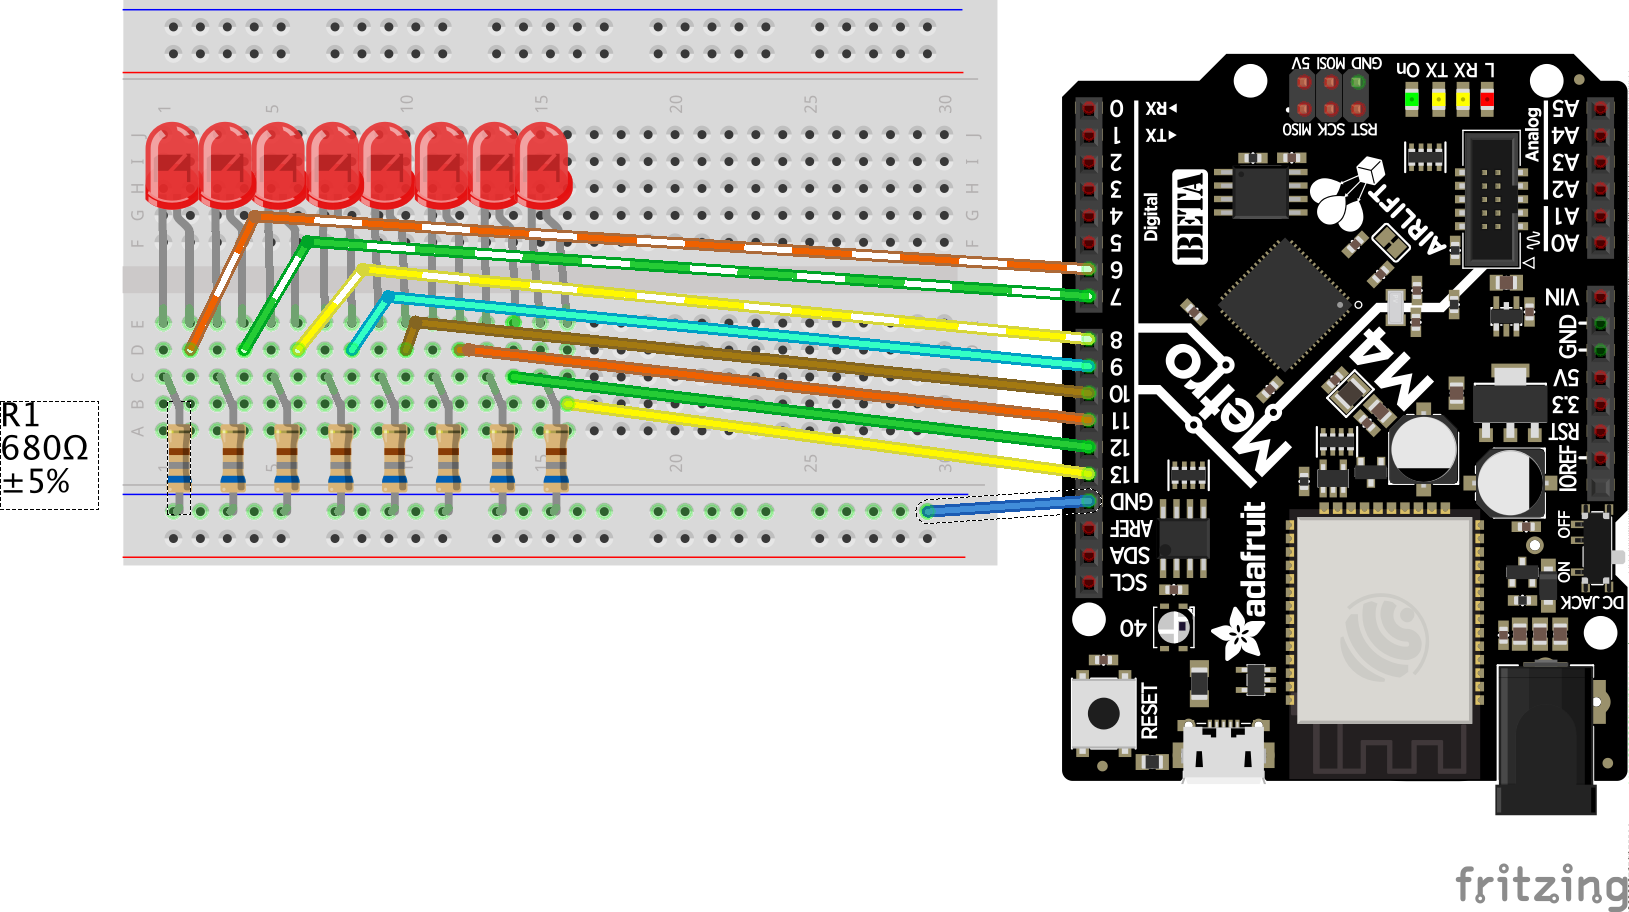
\includegraphics[width=\linewidth]{figures/MultipleLED.png}}
		\caption{Acht Ledjes}
		\label{fig:MultipleLED}
	\end{figure}
\newpage
	\lstinputlisting{code/Multiple_LED.py}
	\paragraph{Discussie:} Voor elk ledje moet 1 pin ge\"initialiseerd worden. Voor 8 ledjes moeten dus 8 pinnen op digitale output gezet worden. Dit gaat hetzelfde als met 1 ledje als in recept~\ref{sec:ledExtern}. Daarna worden alle ledjes in een lijst gezet, zodat met een for loop door de ledjes gelooped kan worden. In de oneindige while loop gaat het programma gelijk de eerste for loop in. Hier worden de ledjes \'e\'en voor \'e\'en aangezet in de volgorde van ledlist met \SI{0.2}{\second} wachtijd tussen elk ledje. Vervolgens gaat het de tweede for loop in, waar de ledjes in omgekeerde volgorde van de ledlist worden uitgezet. 

\newpage
\section{Meerdere LEDjes met minder pinnen door middel van een shiftregister}
	\paragraph{Probleem:} Je wilt meerdere ledjes aansturen, maar wilt niet per ledje 1 pin opofferen.
	\paragraph{Benodigdheden:}
		\begin{itemize}
			\item 8x LED
			\item 8x \SI{680}{\ohm} weerstand (in dit geval mag een lagere weerstand van \SI{220}{\ohm} gebruikt worden omdat de stroom niet door de I/O pinnen wordt geleverd)
			\item 1x SN74HC595N shift register
		\end{itemize}
	\paragraph{Oplossing}:
	\begin{figure}[H]
		\center{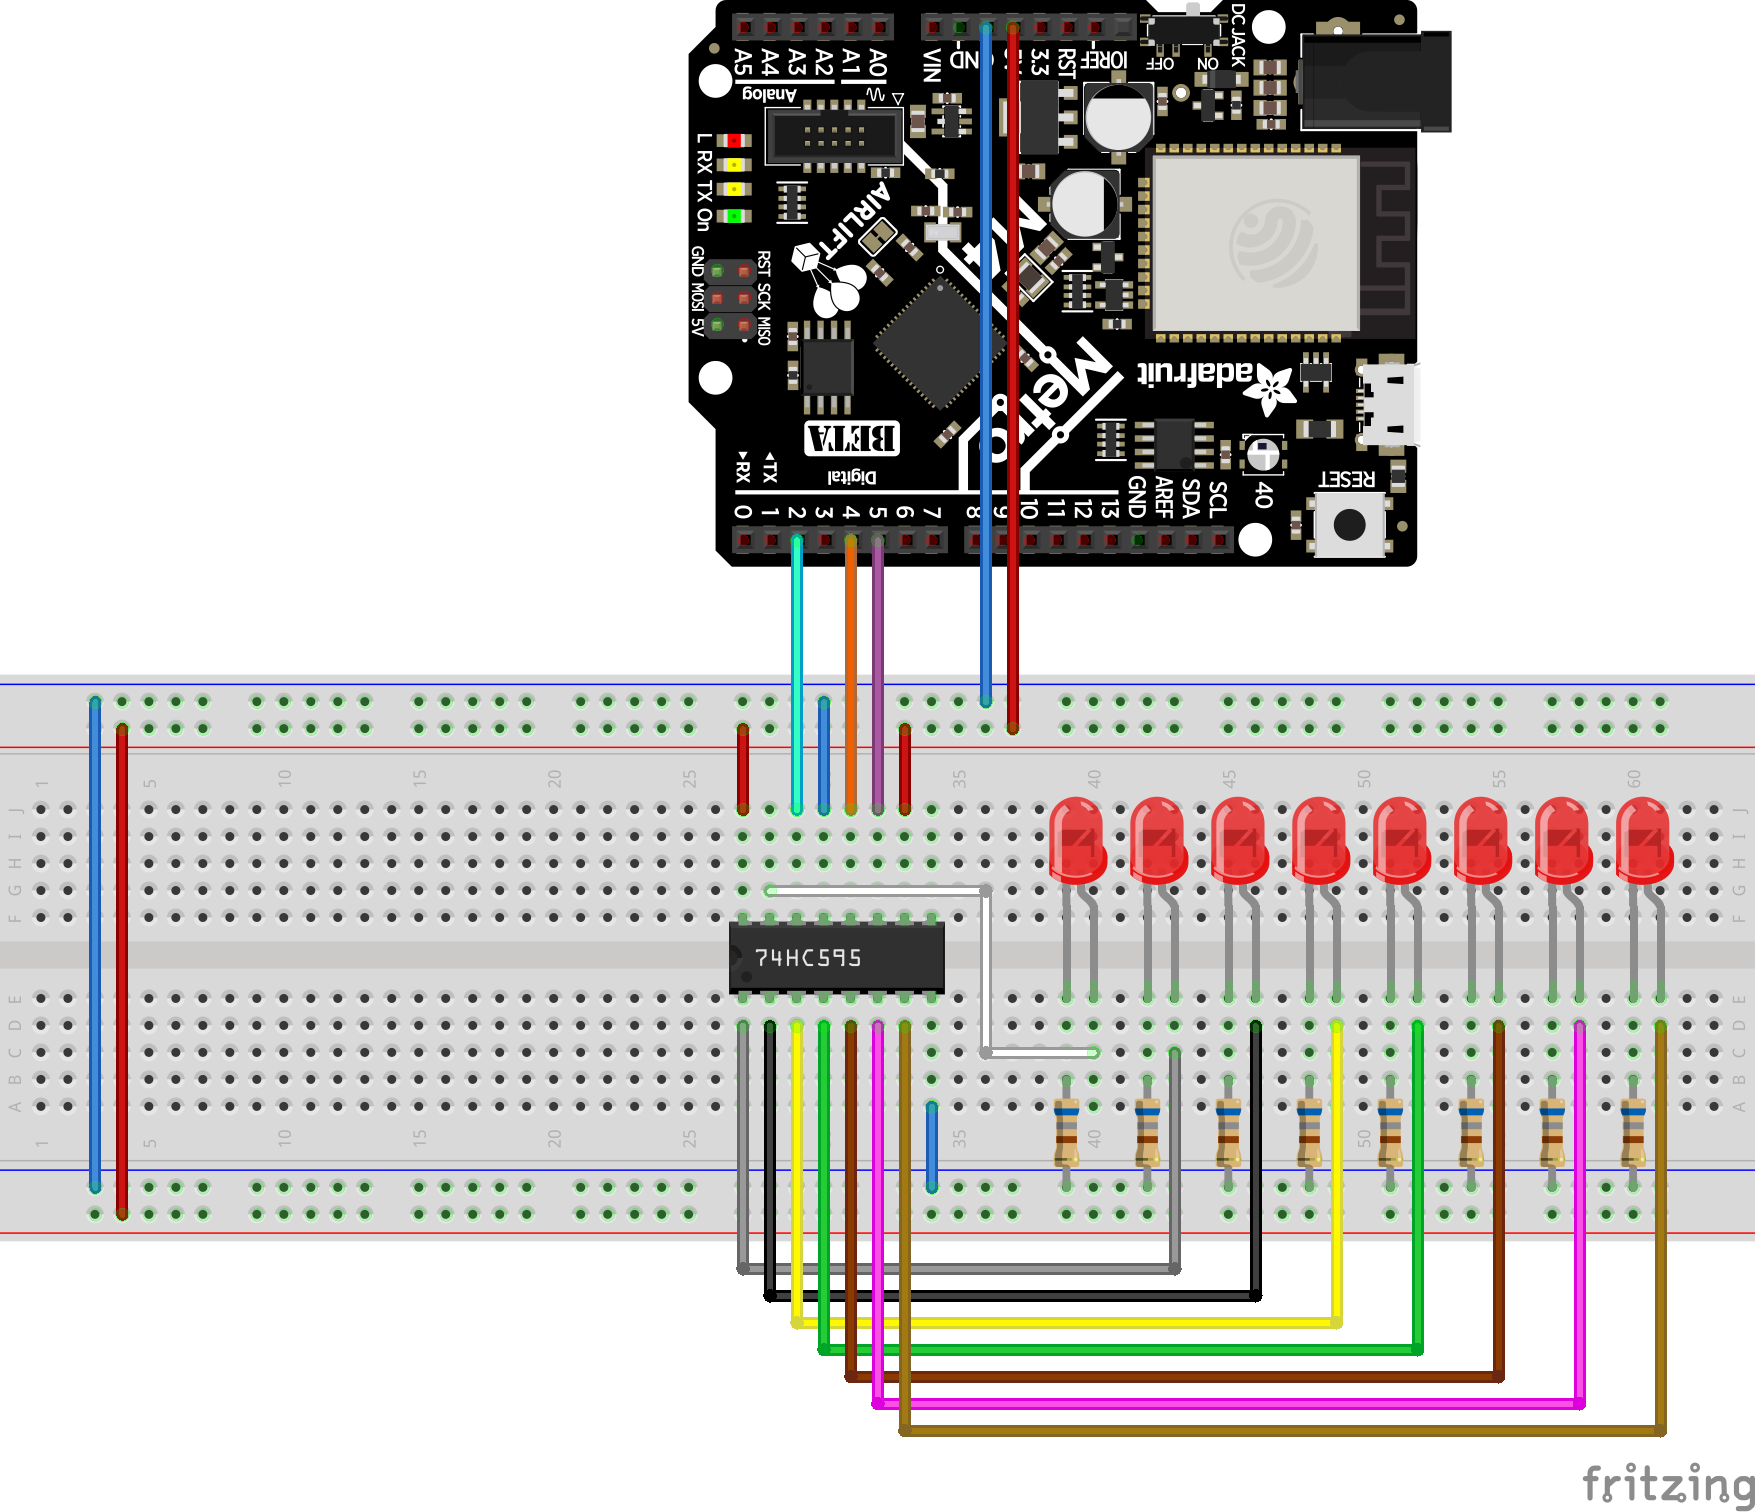
\includegraphics[width=0.75\linewidth]{figures/ShiftRegister.png}}
		\caption{Acht ledjes met een shiftregister}
		\label{fig:ShiftRegister}
	\end{figure}
	
	\clearpage
	\newpage
	
	\lstinputlisting{code/Shiftregister.py}
	\newpage
	\paragraph{Discussie:} Een shiftregister wordt gebruikt om een groot aantal ledjes (of iets anders) aan te sturen, zonder dat je voor elk ledje een nieuwe pin nodig hebt, zoals in recept~\ref{sec:meerdereLedjes}. Je kunt met 3 I/O pinnen een oneindig aantal ledjes aansturen als je meerdere shiftregisters aan elkaar koppelt. Het gebruik van een shiftregister is wel iets complexer. Dus hoe werkt het?
	
	Het schema van het shiftregister is te zien in figuur~\ref{fig:SN74HC595N}. 
	\begin{enumerate}
		\item Qa, Qb.... ,Qh zijn de pinnen waar de ledjes op aangesloten worden.
		\item Vcc en GND zijn de pinnen die de stroom aan zowel de ledjes als de IC leveren.
		\item De $\overline{OE}$ pin schakelt Qa-Qh tegelijk uit als er een hoge spanning op staat. In ons geval is het niet nodig om Qa-Qh tegelijk uit te zetten, dus kan de pin direct op ground aangesloten worden.
		\item De $\overline{SRCLR}$ pin cleared het shift register als er een lage spanning op gezet wordt. Dit is onnodig, dus deze pin wordt aangesloten op 3.3V, net als Vcc.
		\item $Q_{H'}$ kun je gebruiken om meerdere IC's aan elkaar te koppelen, dat hier niet wordt gedaan. Deze kan dus open blijven.
	\end{enumerate}  
	
	De overgebleven SER, RCLK en SRCLK worden gebruikt om Qa-Qh in te stellen, waar de ledjes aan vast zitten. Een shiftregister werkt met het principe van doorschuiven. Het shiftregister heeft 8 stukjes geheugen, \'e\'en register per Q pin. Als de SRCLK pin van een lage naar een hoge spanning gebracht wordt, wordt een 1 of een 0 in het register van Qa gezet, afhankelijk van of de spanning op de SER pin respectievelijk hoog of laag is. Tegelijkertijd schuift de waarde die in het register van Qa stond naar Qb, van Qb naar Qc, etc.. Door de gewenste waardes in de goede volgorde op de SER pin te zetten en de SRCLK van laag naar hoog te brengen kunnen de gewenste waarden in de registers van de Q-pinnen gezet worden. Voordat de waarden actief worden moet de RCLK van laag naar hoog gebracht worden.
	
	Het gebruik van het shiftregister werkt als volgt. Eerst zet je RCLK en SRCLK laag. Wat je als eerst op de SER pin zet bepaald uiteindelijk of de laatste pin $Q_H$ aan of uit gaat staan. Als je het ledje op $Q_H$ aan wilt, zet je een hoge spanning op de SER pin en breng je SRCLK van laag naar hoog. In het register van Qa komt nu een 1. Vervolgens breng je SRCLK weer laag en bepaal je of $Q_G$ aan of uit moet. Als Qh uit moet, zet je een lage spanning op de SER pin en breng je SRCLK weer naar hoog. De 1 van Qa schuift door naar Qb en in Qa komt nu een 0. Dit doe je in totaal acht keer tot alle waarden in de registers staan. Tot slot breng je RCLK van laag naar hoog om het definitief te maken en gaan de gewenste ledjes aan de Q-pinnen branden.
	
	Dit proces is gecodeerd in de writereg() functie. Je geeft de functie een lijst met welke van de Qa-Qh aan en uit moeten. De functie loopt dan van achter naar voren door de lijst, omdat je het laatste ledje als eerste in moet voeren. Als in alle registers de juiste waarde staat wordt een hoge spanning op RCLK gezet om het definitief te maken.


	\begin{figure}[!htb]
		\center{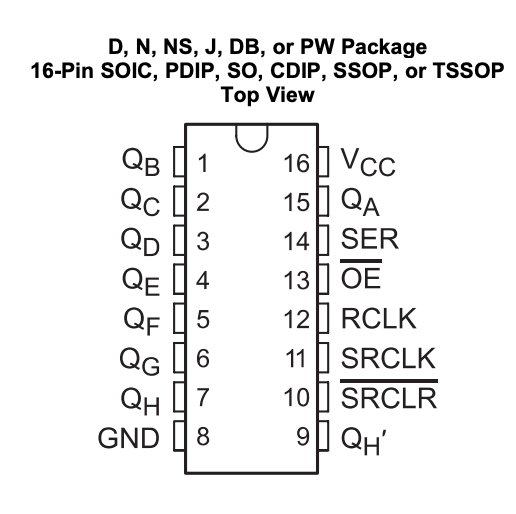
\includegraphics[width=0.5\linewidth]{figures/SN74HC595N.png}}
		\caption{Pin-out diagram van SN74HC595N}
		\label{fig:SN74HC595N}
	\end{figure}

\newpage
\section{Neopixel}
	\paragraph{Probleem:} Je wilt de neopixel (RGB LED) op het bordje gebruiken.
	\paragraph{Oplossing:} CircuitPython heeft een speciale bibliotheek voor het gebruik van de neopixel. Code om de RGB over te laten springen van rood naar groen naar blauw is hieronder te zien.
	\lstinputlisting{code/Neopixel.py}
	
	\paragraph{Discussie:} Zorg er eerst voor dat de neopixel bibliotheek in de lib folder op je bordje staat. Om vervolgens gebruik te maken van de neopixel bibliotheek moet de bibliotheek eerst worden ge\"importeerd. Vervolgens kan gebruik gemaakt worden van de NeoPixel() functie om een NeoPixel object te maken dat controle geeft over de NeoPixel via simpele commando's in de code. De NeoPixel() functie heeft als eerste parameter de I/O pin waar de neopixel op aangesloten is en als tweede parameter het aantal neopixels. In ons geval zit \'e\'en neopixel aangesloten op een interne pin met de naam board.NEOPIXEL. Na het cre\"eren van een neopixel object met de naam 'led', kan de neopixel heel makkelijk worden ingesteld door led aan te roepen in de code. De felheid kan worden ingesteld door led.brightness aan te passen en de kleur van de neopixel kan worden ingesteld door de verhouding van rood/groen/blauw licht in te stellen. Dit kan door elk van de kleuren een waarde tussen de 0 en 255 te geven.
	
	
	\paragraph{Extra informatie over het gebruik van de neopixel}:\\
	
	\url{https://learn.adafruit.com/circuitpython-essentials/circuitpython-internal-rgb-led}
	\url{https://circuitpython.readthedocs.io/projects/neopixel/en/latest/}
	
\section{LCD Screen}
\paragraph{Probleem:} Je wilt tekst naar een LCD screen printen.
\paragraph{Benodigdheden:}
	\begin{itemize}
		\item 1x Bi-Directional Level-Shifter 5-3.3V (Niet nodig maar zorgt voor feller licht)
		\item 1x LCD scherm
		\item 1x PCF8574 i2c LCD controller
	\end{itemize}
\paragraph{Oplossing}:
\begin{figure}[!htb]
	\center{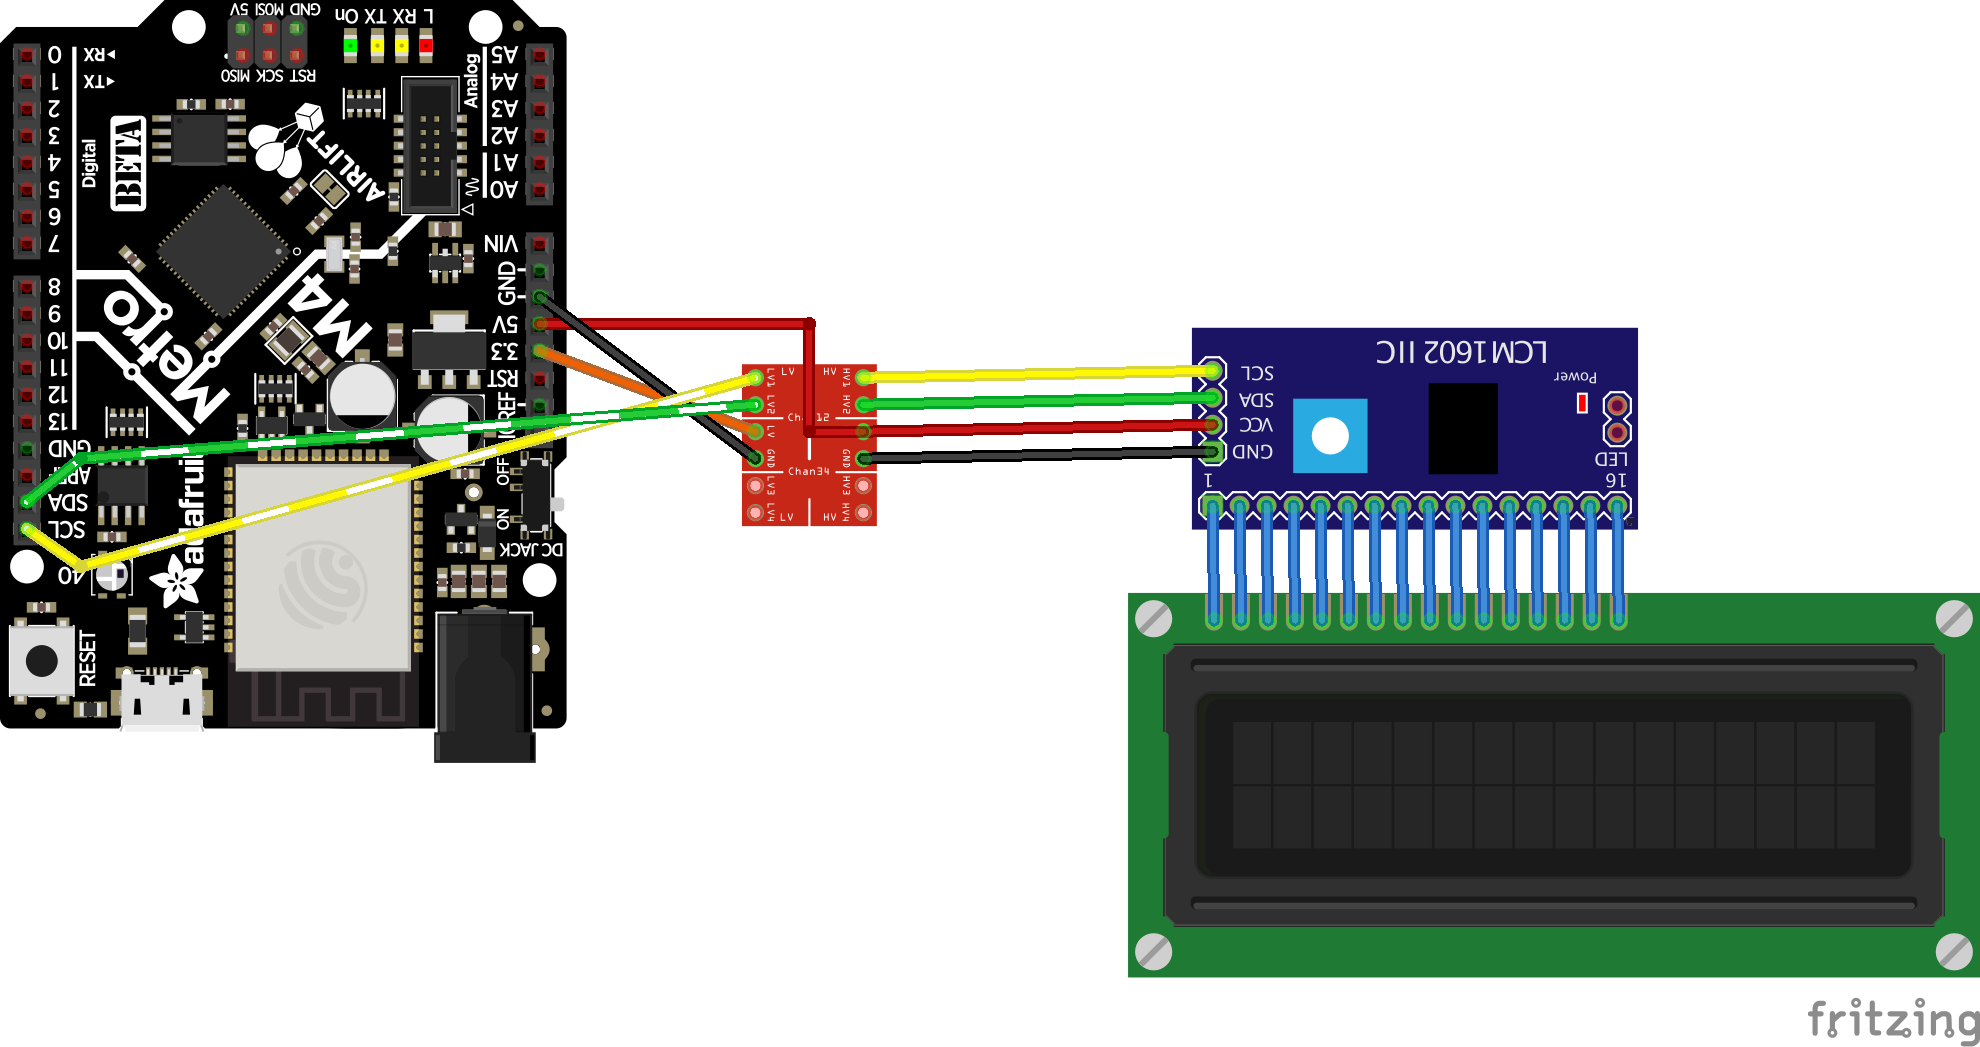
\includegraphics[width=\linewidth]{figures/LCD.png}}
	\caption{LCD Screen Circuit}
	\label{fig:LCD}
\end{figure}
\lstinputlisting{code/LCD.py}
\newpage
\paragraph{Discussie:} Tussen het LCD scherm en het CircuitPython bordje zit een level shifter, omdat het lcd scherm 5V logic gebruikt en het bordje 3.3V. De level shifter heeft een HV en LV pin, waarop de referentie spanning gezet moet worden. Zet op LV dus 3.3V en op HV 5V. De level shifter converteert dan automatisch een spanning van 3.3V op de pinnen LV1-LV4 naar een spanning van 5V op respectivelijk HV1-HV4. De level shifter werkt ook in de andere richting.

Download voor het gebruik van de code eerst de LCD bibliotheek van \url{https://github.com/dhalbert/CircuitPython_LCD} door op \textit{clone or download} en dan \textit{download ZIP} te klikken. Unzip de .zip file en zet het mapje met de naam 'lcd' in de lib folder op je CircuitPython bordje. In de code worden eerst de benodigde modules ge\"importeerd. Daarna wordt een LCD object gemaakt met de naam "lcd". De positie van de cursor kan verplaatst worden met object.set\_cursor\_pos() en er kan tekst geprint worden met object.print(). Met object.clear() wordt het scherm leeg gemaakt en wordt de cursor positie terug naar het begin verplaatst. \\

\clearpage
\newpage

Doet de bibliotheek het niet ? \\

Pas dan de bibliotheek als volgt aan:

\begin{lstlisting}
    def _write4bits(self, value):
        """Pulse the `enable` flag to process value."""
        with self.i2c_device:
            self._i2c_write(value & ~PIN_ENABLE)
            # This 1us delay is probably unnecessary, given the time needed
            # to execute the statements.
            microcontroller.delay_us(1)
            self._i2c_write(value | PIN_ENABLE)
            microcontroller.delay_us(1)
            self._i2c_write(value & ~PIN_ENABLE)
        # Wait for command to complete.
        microcontroller.delay_us(100)
\end{lstlisting}

Voor het volgende stukje code:

\begin{lstlisting}
    def _write4bits(self, value):
        """Pulse the `enable` flag to process value."""
        with self.i2c_device:
            self._i2c_write(value & ~PIN_ENABLE)
            # This 1us delay is probably unnecessary, given the time needed
            # to execute the statements.
            #microcontroller.delay_us(1)
            self._i2c_write(value | PIN_ENABLE)
            #microcontroller.delay_us(1)
            self._i2c_write(value & ~PIN_ENABLE)
        # Wait for command to complete.
        #microcontroller.delay_us(100)
\end{lstlisting}